This section describes the results of the LQ statistical analysis.

\subsection{Fit crosschecks}
\label{subsec:LQ_fitcrosschecks}

\textcolor{red}{To do: investigation of the pull and limit behaviours, especially for the LQ \lephad channel, are ongoing.}

The fit model is validated in various steps.  First, separate fits are performed for the \hadhad and \lephad channels. 
The \hadhad fit includes the \hadhad signal region and the Z+HF control region. The \lephad fit includes the \lephad signal 
region and the Z+HF control region. Second, the combined fit using the \lephad + \hadhad SRs and the Z+HF CR is 
performed. In all fits the normalizations of the $t\bar{t}$ and Z+HF backgrounds are freely floating NPs. 

%Figure~\ref{fig:LQ_CombinedPostfitPNNScoreDistributions} shows the post-fit PNN score distributions for the 300, 500, 1000 and the post-fit SM BDT distribution from the \hadhad background-only fit (these distributions are blinded in the high MVA score region containing 85\% of the signal). The corresponding distributions for the \lephad channel are shown in Fig. \ref{fig:LepHadSLTPostfitPNNScoreDistributions} and \ref{fig:LepHadLTTPostfitPNNScoreDistributions} for the SLT and LTT categories, respectively.

\Cref{fig:LQ_LepHadPostfitPNNScoreDistributions} -~\ref{fig:LQ_CombinedPostfitPNNScoreDistributions} shows the post-fit PNN score 
distributions and $m_{ll}$ distribution of Z+HF CR for the 1400 GeV LQ signal for \hadhad, \lephad, and \lephad + \hadhad combined 
background only fit (these distributions are blinded in the high MVA score region containing 85\% of the signal). 

\begin{figure}
\centering
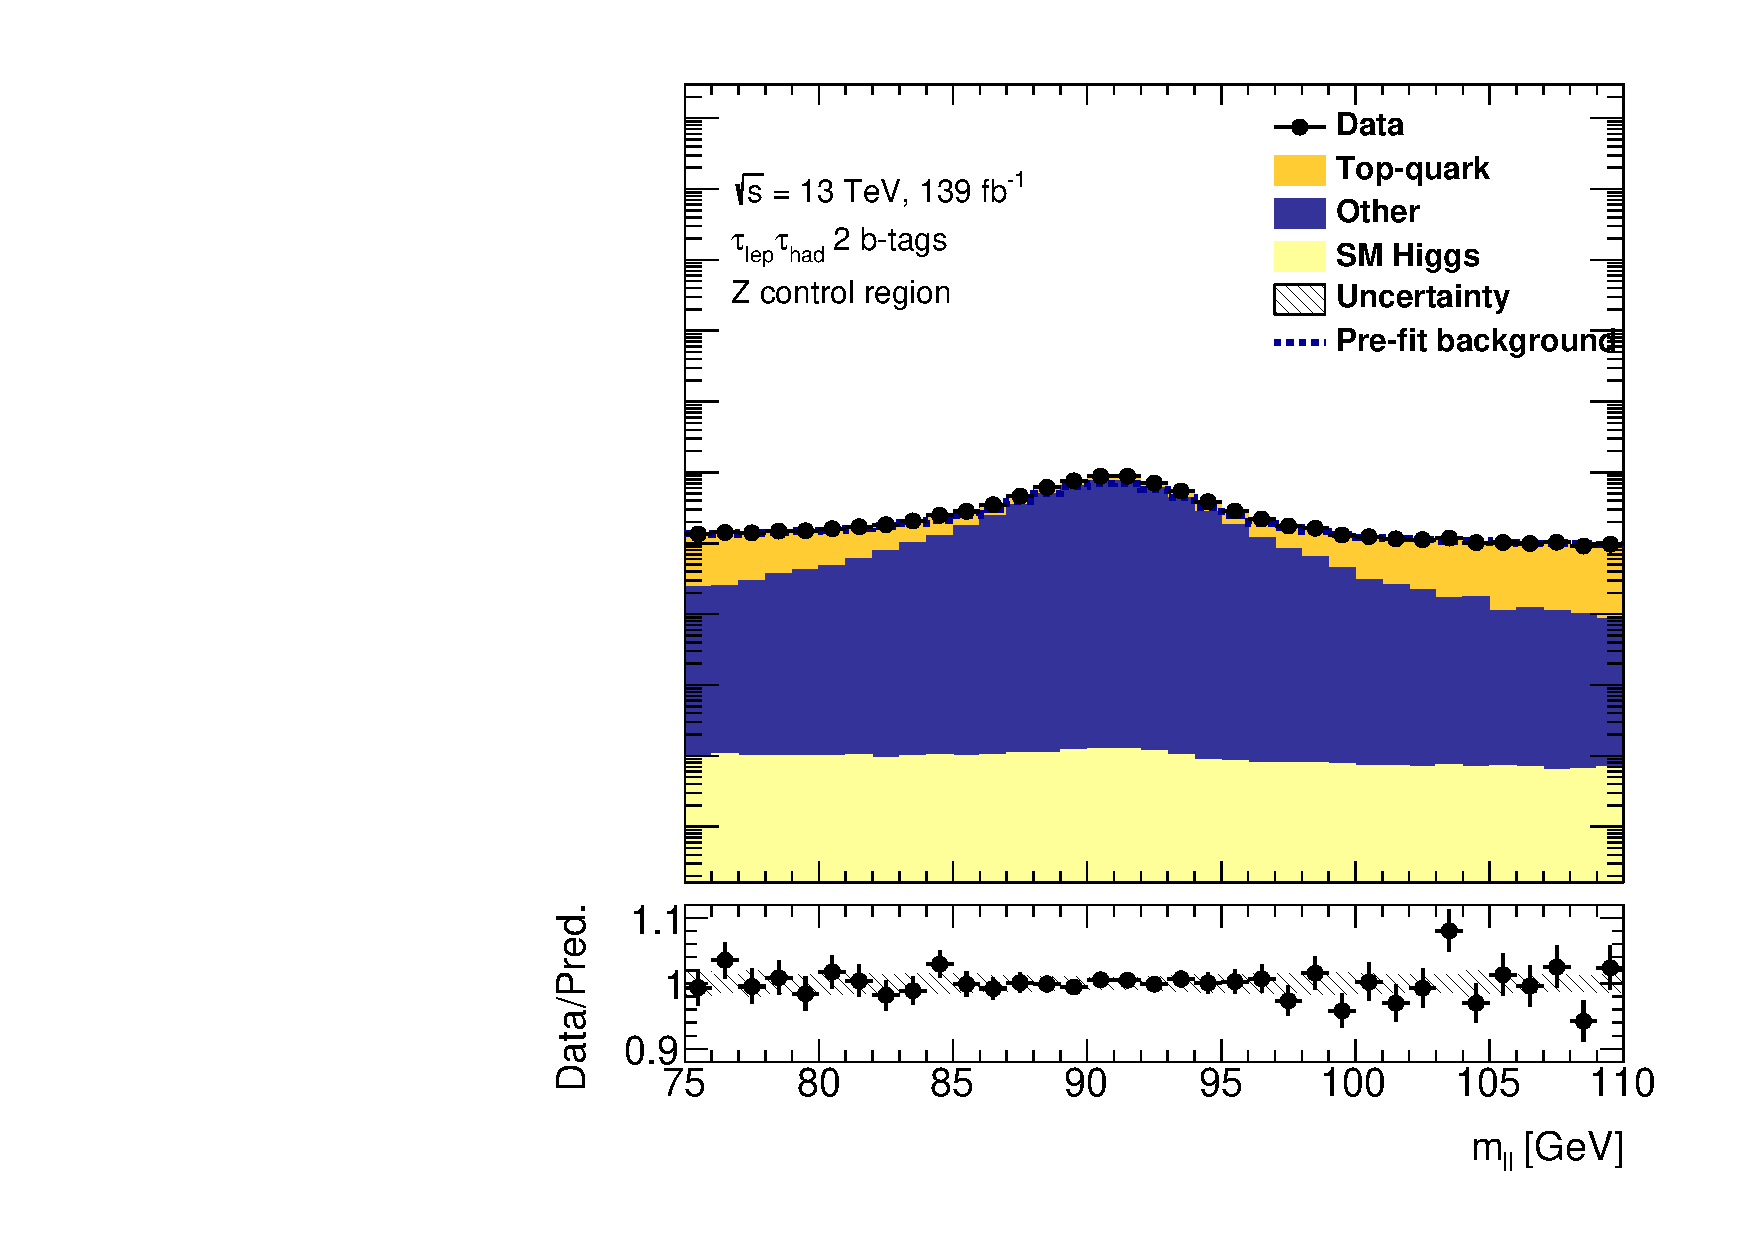
\includegraphics[width=.4\textwidth]{figures/results/LQ/Region_BMin0_incJet1_Y2015_DZllbbCR_T2_L2_distmLL_J2_GlobalFit_conditionnal_mu0log.pdf}
\includegraphics[width=.4\textwidth]{figures/results/LQ/Region_BMin0_incJet1_dist1400_J2_DPNN_T2_SpcTauLH_Y2015_LTT0_L1_GlobalFit_conditionnal_mu0log.pdf}
\caption{Post-fit PNN distribution for the LQ \lephad + Z+HF CR fit to data for the LQ mass of 1400 GeV fit (inputs from 8\textunderscore 3\textunderscore 2021).}
\label{fig:LQ_LepHadPostfitPNNScoreDistributions}
\end{figure}

\begin{figure}
\centering
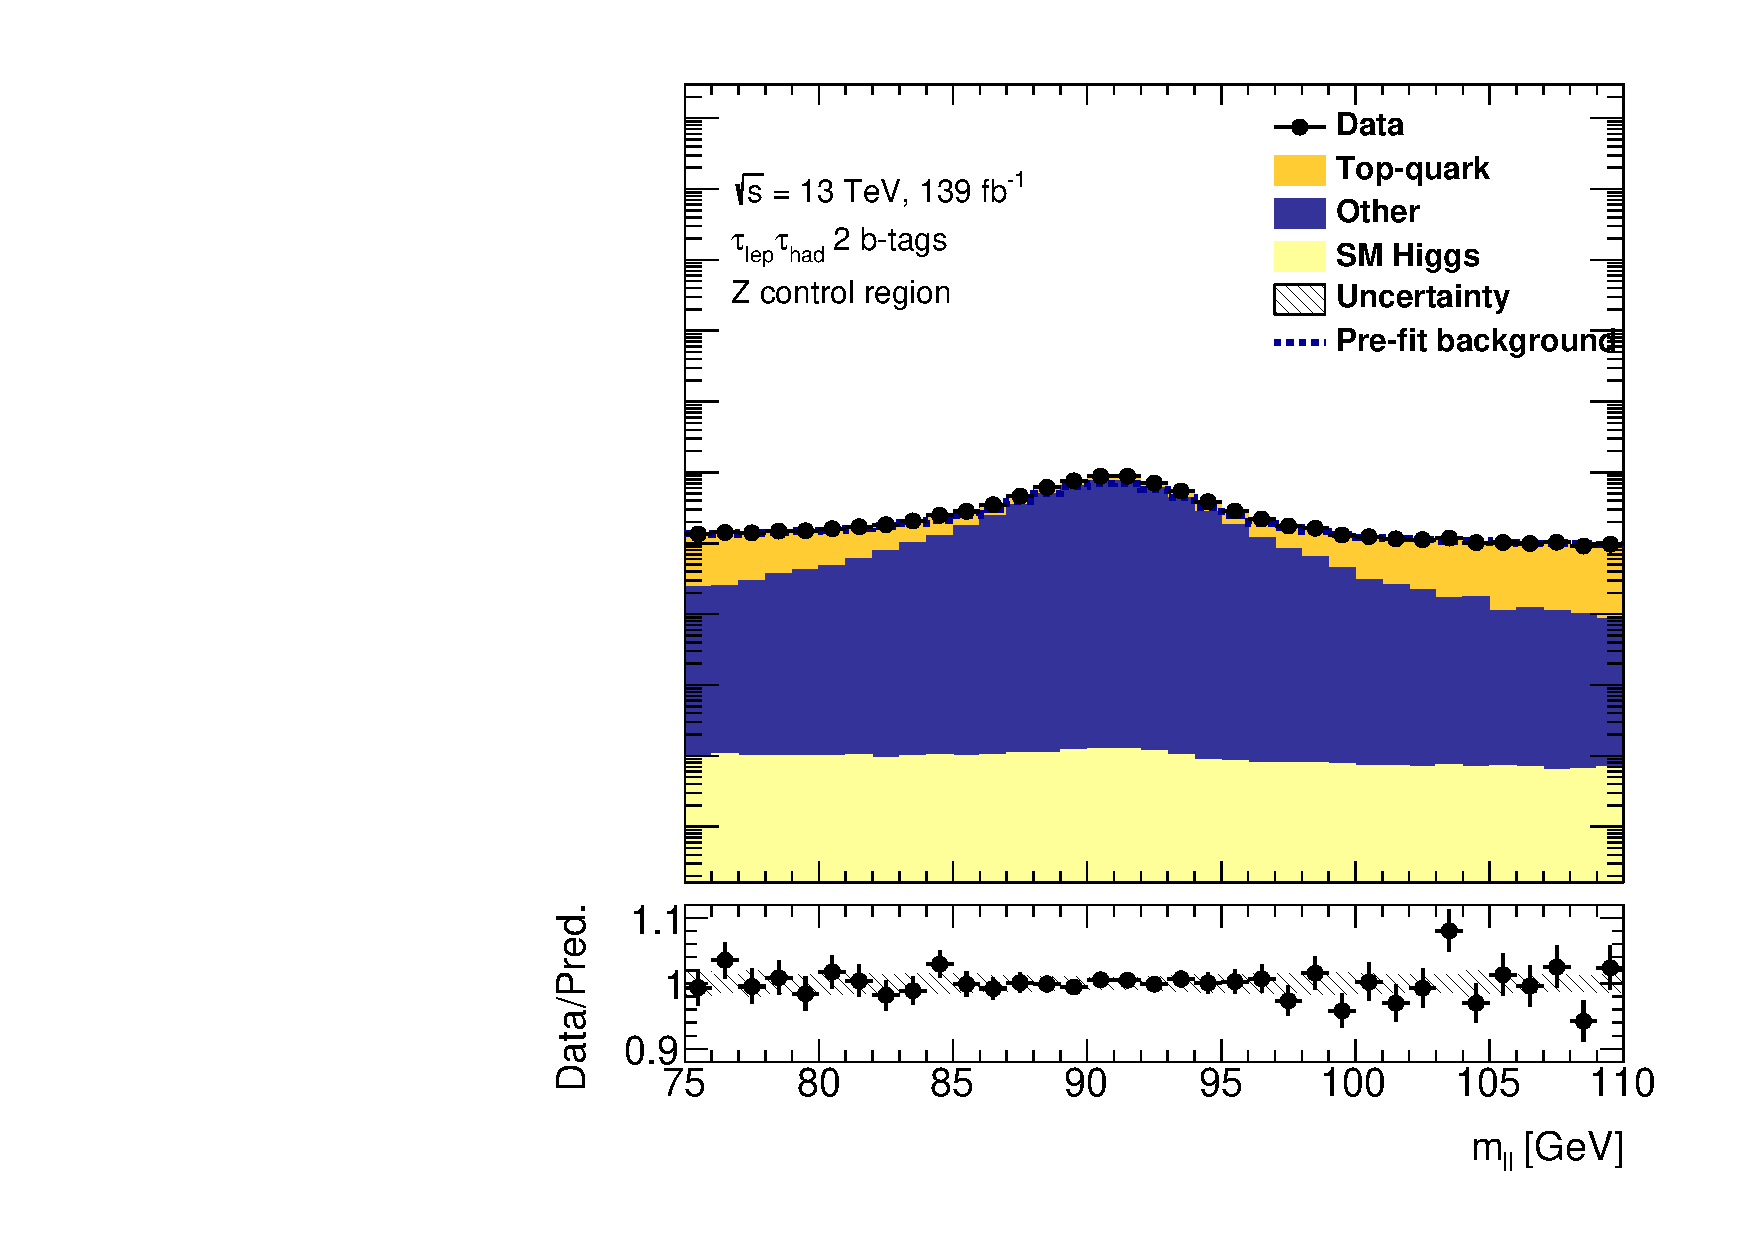
\includegraphics[width=.4\textwidth]{figures/results/LQ/Region_BMin0_incJet1_Y2015_DZllbbCR_T2_L2_distmLL_J2_GlobalFit_conditionnal_mu0log.pdf}
\includegraphics[width=.4\textwidth]{figures/results/LQ/Region_BMin0_incJet1_dist1400_J2_Y2015_DOSSRLQ3PNN0_T3_SpcTauHH_L0_GlobalFit_conditionnal_mu0log.pdf}
\caption{Post-fit PNN distribution for the LQ \hadhad + Z+HF CR fit to data for the LQ mass of 1400 GeV fit (inputs from 8\textunderscore 3\textunderscore 2021).}
\label{fig:LQ_HadHadPostfitPNNScoreDistributions}
\end{figure}

\begin{figure}
\centering
\includegraphics[width=.3\textwidth]{figures/results/LQ/Region_BMin0_incJet1_combined_Y2015_DZllbbCR_T2_L2_distmLL_J2_GlobalFit_conditionnal_mu0log.pdf}
\includegraphics[width=.3\textwidth]{figures/results/LQ/Region_BMin0_incJet1_dist1400_J2_DPNN_T2_SpcTauLH_Y2015_LTT0_L1_GlobalFit_conditionnal_mu0log.pdf}
\includegraphics[width=.3\textwidth]{figures/results/LQ/Region_BMin0_incJet1_dist1400_J2_Y2015_DOSSRLQ3PNN0_T3_SpcTauHH_L0_GlobalFit_conditionnal_mu0log.pdf}
\caption{Post-fit PNN distribution for the LQ \lephad and \hadhad + Z+HF CR combined fit to data for the LQ mass of 
1400 GeV fit (inputs from 8\textunderscore 3\textunderscore 2021).}
\label{fig:LQ_CombinedPostfitPNNScoreDistributions}
\end{figure}

%\Cref{fig:LQ_HadHadPostfitNPRankings500}-~\ref{fig:LQ_HadHadPostfitNPRankings1400} shows the NP pulls for the \hadhad fit for an unconditional fit to the Asimov dataset. % built with $\mu=0$ (red) and to data (black) for the LQ mass of 1400 Gev fits. % Figures \ref{fig:LepHadPostfitNPPulls2HDM300}-~\ref{fig:LepHadPostfitNPPullsSM} show the equivalent NP pulls for the \lephad channel.

\Cref{fig:LQ_LepHadPostfitNPPulls1400} -~\ref{fig:LQ_CombinedPostfitNPPulls1400} show the NP pulls for the \lephad, \hadhad and combined unconditional fits to the Asimov dataset. % built with $\mu=0$ (red) and to data (black) for the LQ mass of 1400 Gev fits. % Figures \ref{fig:LepHadPostfitNPPulls2HDM300}-~\ref{fig:LepHadPostfitNPPullsSM} show the equivalent NP pulls for the \lephad channel.

\begin{figure}
\centering
\includegraphics[width=.7\textwidth]{figures/results/LQ/output_lephad_LQ3_1400_pulls_20210308.pdf}
\caption{NP pull plot for the LQ \lephad + Z+HF CR fit to data for the LQ mass of 1400 GeV fit (inputs from 8\textunderscore 3\textunderscore 2021).}
\label{fig:LQ_LepHadPostfitNPPulls1400}
\end{figure}

\begin{figure}
\centering
\includegraphics[width=.7\textwidth]{figures/results/LQ/output_hadhad_LQ3_1400_pulls_20210308.pdf}
\caption{NP pull plot for the LQ \hadhad + Z+HF CR fit to data for the LQ mass of 1400 GeV fit (inputs from 8\textunderscore 3\textunderscore 2021).}
\label{fig:LQ_HadHadPostfitNPPulls1400}
\end{figure}

\begin{figure}
\centering
\includegraphics[width=.7\textwidth]{figures/results/LQ/output_combined_LQ3_1400_pulls_20210308.pdf}
\caption{NP pull plot for the LQ \lephad and \hadhad + Z+HF CR combined fit to data for the LQ mass of 1400 GeV fit (inputs from 8\textunderscore 3\textunderscore 2021).}
\label{fig:LQ_CombinedPostfitNPPulls1400}
\end{figure}

\Cref{fig:LQ_LepHadPostfitNPRankings1400} -~\ref{fig:LQ_CombinedPostfitNPRankings1400} show the NP rankings for the \lephad, \hadhad and combined 
fits to data for LQ mass of 1400 GeV.

\begin{figure}
\centering
\includegraphics[width=.8\textwidth]{figures/results/LQ/pulls_SigXsecOverSM_lephad_1400_20210308.pdf}
\caption{NP ranking plot for the LQ \lephad + Z+HF CR fit to data for the LQ mass of 1400 GeV fit (inputs from 7\textunderscore 3\textunderscore 2021).}
\label{fig:LQ_LepHadPostfitNPRankings1400}
\end{figure}

\begin{figure}
\centering
\includegraphics[width=.8\textwidth]{figures/results/LQ/pulls_SigXsecOverSM_hadhad_1400_20210307.pdf}
\caption{NP ranking plot for the LQ \hadhad + Z+HF CR fit to data for the LQ mass of 1400 GeV fit (inputs from 7\textunderscore 3\textunderscore 2021).}
\label{fig:LQ_HadHadPostfitNPRankings1400}
\end{figure}

\begin{figure}
\centering
\includegraphics[width=.8\textwidth]{figures/results/LQ/pulls_SigXsecOverSM_combined_1400_20210308.pdf}
\caption{NP ranking plot for the LQ \lephad and \hadhad + Z+HF CR combined fit to data for the LQ mass of 1400 GeV fit (inputs from 7\textunderscore 3\textunderscore 2021).}
\label{fig:LQ_CombinedPostfitNPRankings1400}
\end{figure}


\subsection{Limits}
\label{subsec:LQ_limits}

\Cref{fig:LQLepHadLimits} -~\ref{fig:LQCombinedLimits} show the 95\% C.L. expected limits on the LQ pair production cross section as a function of 
LQ mass from the \lephad, \hadhad, and \lephad and \hadhad combined channels for systematics included and statistical only.

\begin{figure}
\centering
\includegraphics[width=.9\textwidth]{figures/results/LQ/limit_LQlephad_1618_Syst_20210308.eps}
\caption{The 95\% C.L. expected limits on the LQ pair production cross section as a function of the LQ mass from the \lephad channel. The black line shows the expected theory cross section, and the black line shows the expected limit only statistical uncertainties of current analysis of 139~\ifb. (Inputs from 7\textunderscore 3\textunderscore 2021)}
\label{fig:LQLepHadLimits}
\end{figure}

\begin{figure}
\centering
\includegraphics[width=.9\textwidth]{figures/results/LQ/limit_LQhadhad_1618_Syst_20210308.eps}
\caption{The 95\% C.L. expected limits on the LQ pair production cross section as a function of the LQ mass from the \hadhad channel. The black line shows the expected theory cross section, and the black line shows the expected limit only statistical uncertainties of current analysis of 139~\ifb. (Inputs from 7\textunderscore 3\textunderscore 2021)}
\label{fig:LQHadHadLimits}
\end{figure}

\begin{figure}
\centering
\includegraphics[width=.9\textwidth]{figures/results/LQ/limit_LQcombined_1618_Syst_20210308.eps}
\caption{The 95\% C.L. expected limits on the LQ pair production cross section as a function of the LQ mass from the \lephad and \hadhad channels combined. The black line shows the expected theory cross section, and the black line shows the expected limit including systematic uncertainties of current analysis and red line shows statistical only limit of 139~\ifb. (Inputs from 8\textunderscore 3\textunderscore 2021)}
\label{fig:LQCombinedLimits}
\end{figure}

